\chapter{Theoretische Grundlagen}

Im Folgenden sollen die theoretischen Grundlagen für die nachfolgende vergleichende Darstellung der Umsetzung sequentieller Prozesse im REST-Umfeld gelegt werden. Zuerst wird grundsätzlich erklärt, was eine RESTful-API ist und danach wird auf die Umsetzung von REST in ABAP näher erleutert. Abgeschlossen wird der theoretische Teil der Arbeit mit einer Darstellung von Fiori Elements, dem Framework zur Entwicklung von Fiori Apps.

\section{RESTful Application Programming Interface}

Eine API ist eine Schnittstelle, über die verschiedene Softwareanwendungen miteinander kommunizieren können. Die API definiert die Methoden, Protokolle und Tools, die für den Zugriff auf die Funktionen und Daten einer Softwareanwendung verwendet werden können. Somit standardisiert eine API die Kommunikation verschiedener Anwendungen und ermöglicht den Zugriff auf bereitgestellte Daten ohne dass die zugreifende Anwendung die interne Logik oder Implementierung der anderen Anwendung kennen muss.

Eine RESTful-API ist eine spezielle Schnittstelle, die den Designkonventionen nach REST folgt.

Das erste Prinzip ist die Client-Server-Architektur. Das bedeutet, dass die Benutzeroberfläche von den gespeicherten Daten getrennt wird. Die Benutzeroberfläche und Sitzung existiert nur auf dem Client und die gespeicherten Daten oder zur verfügung gestellten Funktionen existieren nur auf dem Server. Somit wird die Portierbarkeit und Skalierbarkeit des Gesamtsystems verbessert. Zudem wird die Möglichkeit einer unabhängigen Weiterentwicklung der verschiedenen Komponenten sichergestellt.

Zudem soll eine RESTful-API zustandslos angelegt sein. Das hei{\ss}t im Genaueren, dass die Kommunikation der verschiedenen Parteien zustandslos sein muss. Es muss für den Server somit möglich sein, die Anfrage des Clients vollständig zu verstehen und zu verarbeiten, ohne zusätzlich auf vergangene Anfragen zugreifen zu müssen. Auf der anderen Seite bedeutet das auch, dass der Client jede Antwort des Servers ohne zusätzliche Inforamtionen, die eventuell zu einem früheren Zeitpunkt angefordert wurden verstehen können muss. Das hei{\ss}t, dass in jeder Anfrage immer alle notwendigen Informationen mitgeschickt werden müssen und von keinem ''Vorwissen'' ausgegangen werden darf. Das hat wiederum zur Folge, dass Sitzungsinformationen ausschlie{\ss}lich auf dem Client gespeichert werden. Durch diese Bedingung verbessert sich die Skalierbarkeit weiter, da der Server Ressourcen, die ansonsten für die Speicherung der Stati der Requests benötigt würden, nicht freihalten muss. Zudem steigt die Zuverlässigkeit der Schnittstelle, da bei einem Fehler immer nur eine Request betrachtet werden muss. Somit ist ein Fehler einfacher behebbar und hat keine Auswirkungen auf andere Anfragen. Damit einher geht auch ein vereinfachtes Monitoring, da immer nur eine Request betrachtet werden muss und nicht erst eine Kette zusammenhängender Anfragen nachvollzogen werden muss.

Die dritte Designkonvention besagt, dass auf der Client Seite ein Cache vorhanden sein muss. Durch das implizite oder explizite Markieren von Daten als cache-fähig dürfen die Anfrage-Daten vom Client für spätere identische Requests wiederverwendet werden. Durch dieses Caching von Daten ist es möglich manche Client-Server Interaktionen teilweise oder ganz zu vermeiden, wodurch die Netzwerkauslastung und Skalierbarkeit verbessert wird. Jedoch birgt die Verwendung eines Caches das Risiko, dass die Daten im Cache im Vergleich zu den auf dem Server gespeicherten Daten schon veraltet sind, was gegebenenfalls zu Fehlern in der weiteren Verarbeitung führen könnte.

Das vierte Prinzip und zentrales Unterscheidungsmerkmal von REST ist das einheitliche Interface zwischen den verschiedenen Komponenten. Hierdurch wird die Systemarchitektur durch das Prinzip der Generalität vereinfacht. Die Schnittstelle ist einfacher benutzbar. Zudem wird eine unabhängige Weiterentwicklung der verschiedenen kommunizierenden Kompoenenten gewährleistet, da die Implementierung der einzelnen Komponenten von den angebotenen Services getrennt wird. Jedoch entsteht durch die einheitliche Schnittstelle auch ein Effizienzverlust, da diese nicht an die Bedürfnisse einer speziellen Anwendung angepasst werden kann.
Um ein einheitliches Interface zu erreichen, finden mehrere Beschränkungen auf die Schnittstelle Anwendung: Ressourcen der Schnittstelle sollen eindeutig identifizierbar sein. Eine Ressource ist eine vom Interface bereitgestellte Information, die eindeutig über einen URI identifizierbar ist. Die Informationen, die durch die Ressourcen repräsentiert werden können statisch festgelegt sein, oder sich auch im Zeitablauf verändern. Zudem kann eine Ressource auch existieren, ohne das die Information schon existiert. Das erleichtert die Verarbeitung verschiedener Informationsarten, da auf abstrakter Ressourcenebene nicht zwischen bestimmten Typen unterschieden wird. Au{\ss}erdem kann so die benötigte Information auch noch zu einem späten Zeitpunkt, je nach Inhalt der Anfrage, festgelegt werden. Zudem hat jeder Service, der nach den REST Prinzipien entworfen ist eine URL, also eine eindeutige Adresse. Durch diese URL ist der Zugriffsweg zum Webservice standardisiert. Durch diese eindeutig identifizierbaren Ressourcen und Services wird zudem die Kombinierbarkeit verschiedener Ressourcen eines Services bzw. von verschiedenen Services in einem grö{\ss}erem System erleichtert. Eine weitere Beschränkung für die Schnittstelle ist die Verwendung von Repräsentationen zur Veränderung von Ressourcen. Eine Repräsentation ist eine Folge von Bytes, die eine Ressource in einer bestimmten Darstellung und zugehörige Metadaten abbildet. Somit kann eine Ressource vom Server in verschiedenen Repräsentationen, je nach Anfrage, zurückgegeben werden. Zudem werden mit der Repräsentation alle Informationen, wie die Ressource verändert werden kann, mitgeschickt. Veränderungen der Ressource finden nur über die Repräsentation statt. Des weiteren sollen Antworten des Servers auf Anfragen selbsterklärend sein. Dass hei{\ss}t, das Standard-Methoden und -Datentypen verwendet werden, um die Ressource zu verändern oder Informationen auszutauschen. Diese Standard-Methoden sind zwar in REST selbst nicht festgelegt, werden aber normalerweise durch die Verwendung des Protokolls auf der Anwendungsschicht definiert. Für das meistens im Internet verwendete HTTP-Protokoll sind diese \zB: GET (gewünschte Ressource vom Server anfordern), POST (neue Ressource unterhalb angegebener Ressource einfügen) oder PUT (angegebene Ressource anlegen bzw. ändern). Die letzte Beschränkung wird als ''Hypermedia as the Engine of Application State'' bezeichnet. Hiermit ist gemeint, dass die Interaktion mit einer API dynamisch über Hypermedien abläuft. Somit ist auf der Client-Seite nur Basiswissen über Hypertext und fast kein Wissen über die Interaktion mit der spezifischen Schnittstelle nötig. Somit können Client und Server voneinander entkoppelt werden, da der Server dem Client neben den angeforderten Informationen dynamisch mögliche Interaktionen zurückgibt.

Die Systemarchitektur soll zudem in Schichten aufgebaut sein. Das hei{\ss}t, dass eine Schicht jeweils nur die nächste darunter- und darüberliegende Schicht sehen und mit ihr interagieren kann. Durch diese Architektur wird die Komplexität des Gesamtsystems reduziert und die unabhängige Weiterentwicklung der einzelnen Schichten gefördert. Zudem können veraltete Dienste abgekapselt werden und und neue somit von diesen getrennt werden. Durch die Aufteilung der Architektur in Schichten kann zudem redundante oder selten benutzte Funktionalität in eine ''Zwischenschicht'' ausgelagert werden. Durch diese Aulagerung verbessert sich zudem die Skalierbarkeit des Systems, da load-balancing, also die Lastverteilung eines Services auf mehrere Netzwerke oder Prozessoren, ermöglicht wird. Dennoch bringt die eine Schichtenarchitektur auch Nachteile mit sich. Durch die Kapselung der Dienste und Funktionalitäten in Schichten steigt der Verwaltungs- und Wartungsaufwand des Gesamtsystems. Zudem sinkt auch die Geschwindigkeit, mit der Daten verarbeitet werden, da die Anfrage im Verarbeitungsprozess wesentlich mehr Schnittstellen passieren muss. Dieser Nachteil kann jedoch durch die Verwendung von geteilten Caches in den Zwischenschichten kompensiert werden, da durch diese Caches die Anzahl der Schnittstellen, die die Anfrage passieren muss, reduziert werden kann. Ein weiterer Vorteil der Schichtenarchitektur ist, dass die Anfragen selektiv von den einzelnen Schichten verändert werden können, da der Inhalt dieser selbst-beschreibend und die Bedeutung der Nachricht für die Zwischenschichten sichtbar ist.

Die sechste (optionale) Designkonvention von REST besagt, dass wenn nötig Code in Form von Skripten oder Apps über die Schnittstelle vom Client heruntergeladen und ausgeführt werden kann. Dies vereinfacht die Programmlogik des Clients, da weniger Programme schon im Voraus vorhanden sein müssen. Zudem wird dadurch die Erweiterbarkeit eines Systems verbessert, da auch nach dem initalen Installieren eines Systems, dieses noch durch das Bereitstellen von Code über die Schnittstelle erweitert werden kann.

\section{ABAP Restful Application Programming Model}

Im Folgenden wird das Restful Application Programming Model für ABAP vorgestellt.

ABAP RAP ist ein Programmiermodell der SAP auf Basis von ABAP, das die Architektur für die Entwicklung von OData-Services, die für die HANA-Datenbank optimiert sind, definiert. Es basiert auf den Designprinzipien nach REST. Mit diesem Modell können sowohl Web APIs veröffentlicht und Business Events erzeugt als auch Fiori Apps entwickelt werden. RAP ist nach dem ''Classic ABAP Programming'' und dem ''ABAP Programming Model for SAP Fiori'' die dritte Evolutionsstufe des ABAP Programming Model.  RAP kann sowohl in Cloud-, als auch in on-premise Systemen eingesetzt werden.

RAP baut im Allgemeinen auf drei Säulen auf: Anders als in den vorhergehenden Programmiermodellen, wo mehrere Tools zum entwickeln von \zB einer Fiori App nötig waren, sind sollen in RAP Implementierungsaufgaben in einer Entwicklungsumgebung integriert werden um einen standardisierteren Entwicklungsprozess zu gewährleisten und diesen für den Entwickler zu vereinfachen. Die zweite Säule ist die Programmiersprache ABAP: Durch Erweiterungen und Anpassungen ist es möglich diese für die Entwicklung mit RAP zu verwenden. Hierbei kommen Technologien wie CDS-Views zum Einsatz um aussagekräftige Daten-Modelle zu definieren. Zudem können vorgefertigte APIs für generische Entwicklungsaufgaben verwendet werden. Die dritte Säule sind umfassende Frameworks, die dem Entwickler helfen, effizient und in kurzer Zeit eine Anwendung zu entwickeln, da einzelne Bausteine automatisch generiert werden können und an bestimmten Stellen noch anwendungsspezifische Logik eingefügt werden kann.

Die Architektur eines OData-Services unter Verwendung von RAP wird nachfolgend beschrieben.

\begin{figure}[h]
    \centering
    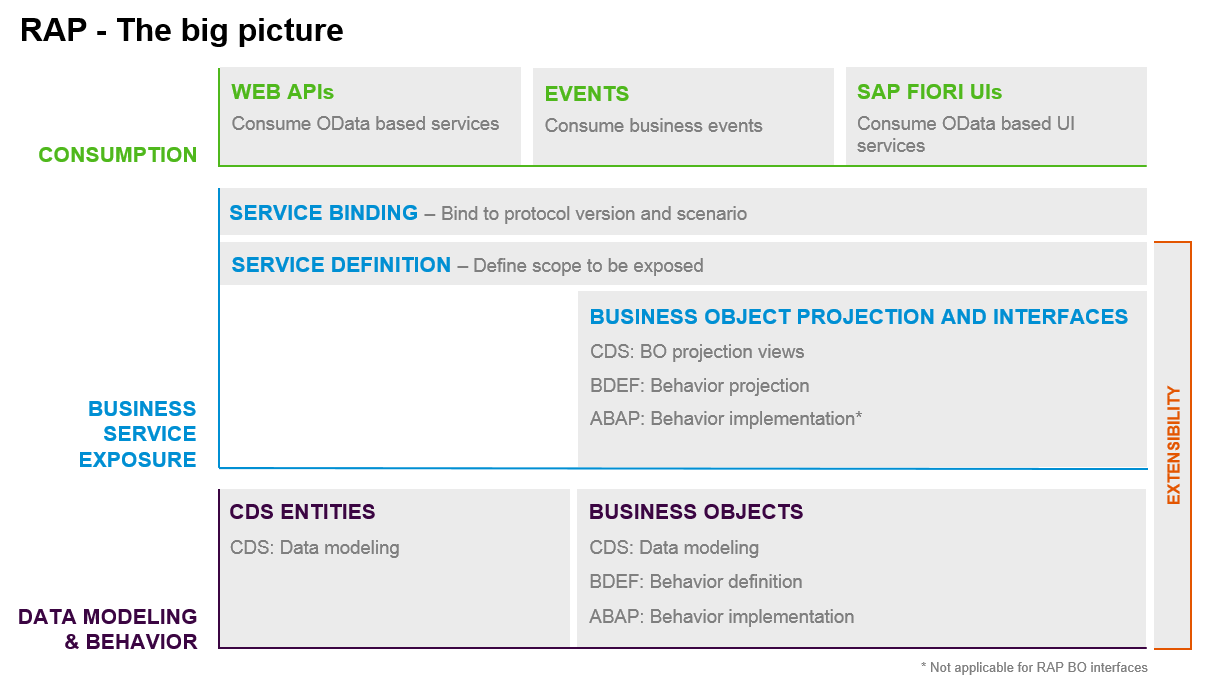
\includegraphics[height=8cm]{Bilder/RAP_Architektur.png}
    \caption[RESTful Application Programming Model Architektur]{RESTful Application Programming Model Architektur}
    \label{fig:iso_norm}
\end{figure}

Auf der untersten Ebene werden die benötigen Daten und das beabsichtigte Verhalten modelliert. Dies kann entweder durch CDS-Views oder durch Business Objects geschehen. Core Data Services sind ein Framework um das Datenmodell, basierend auf der HANA-Datenbank, zu definieren und zu organisieren. Es können selektiv die benötigten Daten aus den Datenbanktabellen ausgewählt werden. Genauer werden alle benötigten Spalten aus einer oder mehreren Tabellen ausgewählt und diese bei Bedarf  mit Annotationen versehen, um speziellere Anforderungen zu erfüllen. Es kann bei Bedarf auch noch nach Datensätzen, die gewisse Bedingungen erfüllen gefiltert werden. Somit strukturiert und gruppiert ein CDS-View die benötigten Daten. Die SQL-Abfrage, um diese Daten von der Datenbank abzurufen ist in dem CDS-View integriert. Der Zweck eines CDS-Views ist jedoch lediglich das Lesen und Strukturieren der Daten; es können hiermit keine Daten verändert werden.

Eine andere Möglichkeit ein Datenmodell zu erzeugen sind Business Objects. Diese bieten zudem die Implementierung von Behaviors (Verhalten) und einer Laufzeit. Ein BO ist aus struktureller Sicht ein hierarchisch aufgebauter Baum aus mehreren Knoten, die gewissen Daten entsprechen und durch Eltern-Kind-Beziehungen (sogenannte Kompositionen) miteinander verknüpft sind. Diese Knoten werden durch CDS Entitäten dargestellt. Der hierarchisch oberste Wurzelknoten stellt dabei die Repräsentation des BO an sich dar. Um das Verhalten eines BO zu spezifizieren, muss eine ''Business Object Behavior definition'' (''Behavior definition'' abgekürzt) angelegt werden. Dieses ABAP Objekt beschreibt das gewünschte Verhalten des BO in RAP. Die Behavior definition bezieht sich immer auf die Wurzel-CDS-Entität eines BO. Diese Behavior definition wird als ABAP Klasse implementiert. Ein Verhalten beschreibt welche Operationen und Feldeigenschaften für ein BO verfügbar sein sollen. Es besteht au{\ss}erdem noch aus der ''Behavior characteristic'', die zusätzliche Eigenschaften, wie \zB Autorisierungen für Operationen festlegt. Operationen sind \zB create() für das Erstellen, update() für das Aktualisieren und delete() für das Löschen eines Datensatzes. Diese modify-Operationen verändern im Gegensatz zu den read-Operationen auch die tatsächlichen Daten auf der Datenbank. Die Laufzeit eines BO besteht aus 2 Teilen: In der Interaktionsphase werden durch das Ausführen von Operationen Daten gelesen und/ oder verändert. Diese Veränderungen werden zunächst in einem ''transactional buffer'' (Pufferspeicher) gespeichert und nachdem alle Änderungen durchgeführt wurden in der sog. ''save sequence'' auf der Datenbank persistiert.

Die zweite Ebene sorgt für das projizieren und von BOs und die Erstellung sowie Veröffentlichung von Business Services. Ein Business Service ist in RAP ein RESTful Service, der Repräsentationen von Ressourcen veröffentlicht, die dann von Konsumenten abgerufen werden können. Die Bestandteile eines Business Services werden später noch genauer erläutert. Die Projektion eines BO ist notwendig, um es flexibel konsumieren zu können, da dieses an sich komplett unabhängig vom OData-Service ist. Das BO an sich stellt die maximal möglichen Funktionen und Daten bereit, die service-unabhängig implementiert und ggf. durch die Projektion auf die für den Service relevanten Aktionen und Daten eingeschränkt werden. Zudem können genauere Anpassungen \zB im Bezug auf die Darstellung auf einer Benutzeroberfläche über UI-Annotationen erfolgen, die aber nicht Teil des Datenmodells sein sollen. Eine zusätzliche Projektions-Schicht hat mehrere Vorteile: Zum einen kann das zugrundeliegende BO angepasst und erweitert werden, ohne dass der darauf aufbauende Service davon betroffen ist. Zum anderen können verschiedene Projektions-Views für verschiedene Anforderungen erstellt werden, die alle dasselbe BO wiederverwenden. Zudem können die Daten und Funktionen eines Services für eine Fiori App oder Web API veröffentlicht werden. Des Weiteren können Services auch rollenbaisert veröffentlicht werden, sodass unterschiedliche Daten und Funktionen für unterschiedliche Anwender bereitgestellt werden können. Um eine solche Projektionsschicht zu erstellen, muss zusätzlich eine CDS Projection View erstellt werden, um die speziellen Daten einer Projektion darzustellen. Dieser basiert auf der CDS View des BO und erzeugt selbst keine neue SQL-View, sondern nur eine Repräsentation der dargestellten Entitäten. Um eine CDS-Entität eines BO zu projizieren müssen die Wurzel-Entität sowie alle Eltern-Entitäten ebenfalls projiziert sein. Zudem wird auch eine Projection Behavior Definition benötigt, die alle Verhalten, die für einen speziellen Service veröffentlicht werden sollen projiziert.

Nachdem Teile des BO projiziert wurden und die zugehörigen Artefakte erstellt wurden, muss in der zweiten Ebene ein Service definiert werden. In einer ''business service definition'' (abgekürzt ''Service Definition'') wird festgelegt, welche CDS Entitäten eines Datenmodells, also welche Daten, in einen bestimmten Service veröffentlicht werden sollen. Die Service Definition stellt eine protokoll-unabhängige und Konsumenten-spezifische Sichtweise auf das Datenmodell dar. Es können auch mehrere CDS-Entitäten oder eine komplette BO Struktur in einem Service veröffentlicht werden. Dafür muss in der Service Definition die hierarchisch höchste Entität des BO, die veröffentlicht werden soll, markiert werden. Diese dient dann als Einstiegspunkt für den Service.

Als letzter Schritt in der zweiten Ebene muss noch das Kommunikationsprotokoll des Service im Service Binding definiert werden. Ein häufiges Beispiel wäre hierbei OData, für das Bereitstellen von Daten in einer Fiori App. Ein Service Binding bezieht sich immer direkt auf eine oder mehrere Service Definitions. Es können auch mehrere Service Bindings basierend auf einer Service Definition erstellt werden. Das ist \zB hilfreich, wenn derselbe Service mit unterschiedlichen Kommunikationsprotokollen veröffentlicht werden soll, da durch die Trennung von Service Definition und Binding das Protokoll von der Geschäftslogik getrennt wird. Somit kann der Entwicklungsaufwand für einen Service erheblich reduziert werden. Ein Service kann für die Protokolle OData Version 2 und 4 veröffentlicht werden, wenn das Ziel ist, die Daten in einer Fiori App darzustellen. OData ermöglicht au{\ss}erdem das Erstellen von HTTP-basierten Services, deren Ressourcen über URIs identifizierbar sind und über HTTP-Nachrichten abgerufen und modifiziert werden können. Dies korrespondiert wiederum mit den Designkonventionen nach REST aus dem vorhergehenden Kapitel. Zudem stehen noch die Protokolle Information Access für Analysezwecke und SQL zur Verfügung. Ein Service kann grundlegend auf zwei Arten veröffentlicht werden: Entweder als UI Service mit den Protokollen OData oder Information Access, indem man dem durch UI-Annotationen eine Fiori Elements oder andere Benutzeroberfläche hinzufügt. Für alle anderen Anwendungsfälle wird der Service als Web API veröffentlicht, die von Clients über das Web mit OData konsumiert werden kann. Wenn ein Service veröffentlicht ist, kann er jedoch im Standard nur innerhalb des Entwicklungssystems abgerufen werden. Ein Service kann zudem in mehreren Versionen existieren. Dies geschieht durch das Hinzufügen oder Entfernen von zusätzlichen Service Definitions zu einem Service Binding. Damit kann ein Service geändert oder erweitert werden.

Die dritte und oberste Ebene der RAP Architektur ist für das Konsumieren der Daten eines BO oder CDS Views verantwortlich. Es gibt zwei Möglichkeiten, diese Daten durch einen Service zu konsumieren. Die erste Möglichkeit ist durch eine Web API. Die Metadaten eines so veröffentlichten Services enthalten keine Informationen über eine Benutzeroberfläche für die Darstellung der Informationen. Der Zugriff auf die bereitgestellten Daten erfolgt über eine öffentliche Schnittstelle des OData Services. Eine weitere Möglichkeit einen Service zu konsumieren ist innerhalb einer Fiori Elements Anwendung als UI Service. Hier werden die Konfigurationen für die Benutzeroberfläche und das Front-End der Anwendung, die im Back-End als Annotationen in den CDS Entitäten festgelegt wurden, über die Metadaten mitgegeben. Somit kann das Fiori Elements Framework aus diesen Metadaten direkt eine fertige UI generieren. Als letzte Möglichkeit ein BO zu konsumieren sind noch Business Events zu nennen. Diese werden hier nur kurz genannt und in einem späteren Kapitel detaillierter beschreiben.

\section{SAP Fiori Elements}

Fiori Elements ist ein Framework zum entwickeln benutzerfreundlicher und ansprechender Anwendungen. Apps werden auf Basis von OData-Services und UI-Annotationen in den CDS Entitäten durch ein umfassendes Framework fast automatisch generiert. Somit ist im Gegensatz zur älteren SAP UI5 Freestyle Technologie kein JavaScript Coding mehr nötig um das Front-End zu programmieren. Elements benutzt vordefinierte Layouts und Controller für Aktionen der App.

Fiori Elements bietet drei zentrale Vorteile: Es soll dabei helfen, dass sich Entwickler auf die spezifische Geschäftsprozess-Logik und die Back-End Entwicklung fokussieren und somit weniger Zeit für die Programmierung der Benutzeroberfläche benötigen, was insgesamt zu einer verkürzten Entwicklungszeit von Apps und somit auch für niedrigere Entwicklungskosten sorgt. Zudem wird die Kontinuität des UI über alle Fiori Apps hinweg und die Übereinstimmung der Apps mit den SAP Designkonventionen sichergestellt. Die Benutzer der Apps haben so eine einheitliche Benutzungserfahrung (Layout, Navigation, Suche, ...) über alle Apps hinweg. Zudem stellt das zentrale Framework auch sicher, dass der Programmcode für die Benutzeroberflächen der Apps immer sofort funktioniert und bietet au{\ss}erdem weitere Funktionen wie Übersetzungen und Unterstützung für mobile Entgeräte. Diese Vorteile tragen wiederum zu einer reduzierten Entwicklungszeit und somit einem Kostenersparnis bei.

Verglichen mit SAP UI5 Freestyle (Freestyle abgekürzt), der anderen Technologie, um Fiori Apps zu entwicklen, lassen sich folgende Unterschiede feststellen: Die generelle Herangehensweise bei Fiori Elements zielt eher auf das effiziente und schnelle Entwickeln und Veröffentlichen einer App ab. Im Gegensatz dazu, liegt der Fokus bei Freestyle eher auf der Flexibilität, spezielle Anforderungen, die ggf. auch nicht mit dem Elements Standard übereinstimmen abbilden zu können. Das wirkt sich auch auf die Möglichkeiten im UI-Design aus: In Fiori Elements ist der Entwickler an die vordefinierten SAP Vorlagen gebunden, während es bei den Freestyle Designs auch möglich ist, mit einer leeren Vorlage zu beginnen. Das hat aber auch zur Folge, dass bei Freestyle wesentlich mehr Webentwicklungs Kenntnisse nötig sind, da die Oberfläche mithilfe von JavaScript Coding selbst programmiert werden muss. In Fiori Elements hingegen wird die gesamte Oberfläche vom Elements Framework generiert und muss nur durch UI-Annotationen in den CDS-Entitäten an die Wünsche des Kunden angepasst werden. Was die Wartbarkeit und entwicklungstechnischen Freiheiten der beiden Technologien angeht, sind auch bei Freestyle grö{\ss}ere Spielräume vorhanden: Dadurch, dass die Oberfläche selbst programmiert wird, ist es möglich eine Logik in das Front-End einzubauen. Diese Tatsache ist für die Problemstellung der Arbeit sehr relevant, da sequentielle Prozesse, die asynchrone Kommunikation benötigen, sich durch eben diese Logik leicht abbilden lassen. Da in Fiori Elements die das UI generiert wird und die Logik von SAP kommt, fehlt diese Gestaltungsmöglichkeit, was die Umsetzung der angesprochenen Geschäftsprozesse erschwert. Dennoch muss man sagen, dass in allen anderen Fällen Fiori Elements erhebliche Vorteile bietet, da bei der Entwicklung einer App sehr viel Zeit und somit auch Geld gespart werden kann, was somit auch die TCO reduziert. 

Beide Fiori Technologien, Elements und Freestyle verwenden das Model-View-Controller Konzept.

\begin{figure}[H]
    \centering
    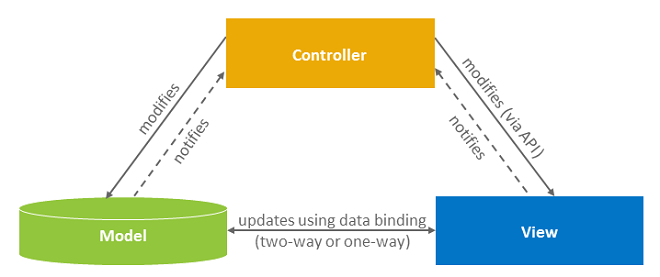
\includegraphics[height=6cm]{Bilder/Fiori_Model-View-Controller-Konzept.png}
    \caption[Model-View-Controller Konzept]{Model-View-Controller Konzept}
    \label{fig:iso_norm}
\end{figure}

Das Konzept unterteilt eine Anwendung in ein Modell, einen View und einen Controller. Das Model verwaltet die Daten der Anwendung und stellt Methoden bereit, um die Daten aus der Datenbank abzurufen und bei Bedarf zu bearbeiten. Fiori unterstützt Client- und serverseitige Modelle. Das hei{\ss}t, dass das Modell entweder komplett vom Client heruntergeladen wird und dort dann lokal existiert, oder bei serverseitigen Modellen nur die jeweils angefragten Daten vom Client beim Server angefordert werden. Wenn das Modell auf der Client Seite existieren soll, kann entweder ein JSON-, XML- oder Ressourcen-Modell verwendet werden. Serverseitig kann ein OData-Service in den Versionen zwei und vier verwendet werden. Es ist auch möglich für verschiedene Bereiche einer Anwendung jeweils verschiedene Modelle zu definieren und diesen auch modellspezifisch über den Controller verschiedene Interaktionsmöglichkeiten mit dem View zu geben. Der View definiert und rendert die Benutzeroberfläche und legt somit das Aussehen der App für den Anwender fest und visualisiert die Daten des Models. Standardmä{\ss}ig werden XML- und JSON-Views unterstützt. Zudem kann man einen View als eigene Klasse selbst programmieren. Der Controller ist für die Interaktionen des Benutzers mit der App zuständig und enthält Methoden, die die Interaktion zwischen Model und View regeln. Er enthält den Programmcode für die Geschäftsprozesslogik hinter der Anwendung. Zudem kann der Controller in Methoden oder zu bestimmten Zeitpunkten, wie \zB bei Start oder Beenden der Anwendung Events auslösen. Diese Events können dann von anderen Controllern empfangen und verarbeitet werden. Somit können eventgesteuert bestimmte Aktionen in der Anwendung ausgelöst werden. Das Ziel des Konzepts ist es, die Daten der App logisch von den Interaktionen des Benutzers zu trennen. Eine Anwendung in die genannten drei Teile aufzuteilen hat folgende Vorteile: Der Programmcode der Anwendung ist leichter lesbar, wartbar und erweiterbar, da er in logisch zusammenhängende Teile aufgeteilt ist. Somit ist es möglich die Darstellung der Daten in der View zu verändern, ohne die darunterliegende Logik oder das Datenmodell zu ändern und mit mehreren Views mehrere Darstellungsweisen, je nach Anwendungsfall zu erstellen.

Apps sind in Fiori Elements immer auf vordefinierten Layouts aufgebaut. Diese können am Anfang der Entwicklung einer App ausgewählt werden und geben das generelle Aussehen und Funktionen vor.

\begin{figure}[H]
    \centering
    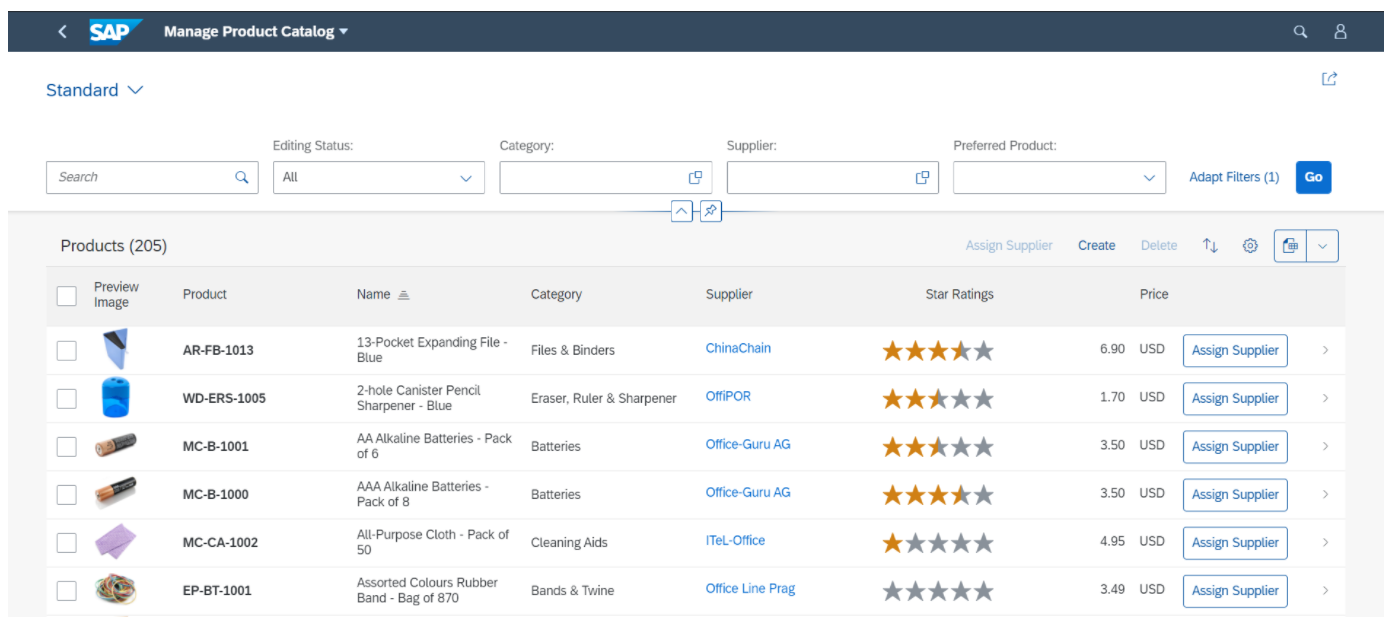
\includegraphics[height=6cm]{Bilder/Fiori_Elements_List_Floorplan.png}
    \caption[Fiori Elements List Report Floorplan]{Fiori Elements List Report Floorplan}
    \label{fig:iso_norm}
\end{figure}

Auf dem Bild ist beispielhaft das Layout List Report zu sehen. Dieser kann verwendet werden, wenn der Zweck der Anwendung das Arbeiten mit einer Liste von Dingen \zB Produkten ist. Diese werden dann in einer sortierten Tabelle dargestellt, in der der Benutzer nach Einträgen sortieren, filtern und suchen kann. Hier müssen nur die Produktdaten über einen OData Service bereitgestellt werden und die Darstellung der Daten über UI-Annotationen nach Bedarf angepasst werden. Die restliche Benutzeroberfläche mit Navigation, Suchleisten und Aktionen wird vollständig durch das Framework generiert. Der List Report wird häufig als Einstiegspunkt in einer App verwendet um nach bestimmten Objekten zu suchen und mit diesen dann in einer Object Page näher zu interagieren.

\begin{figure}[H]
    \centering
    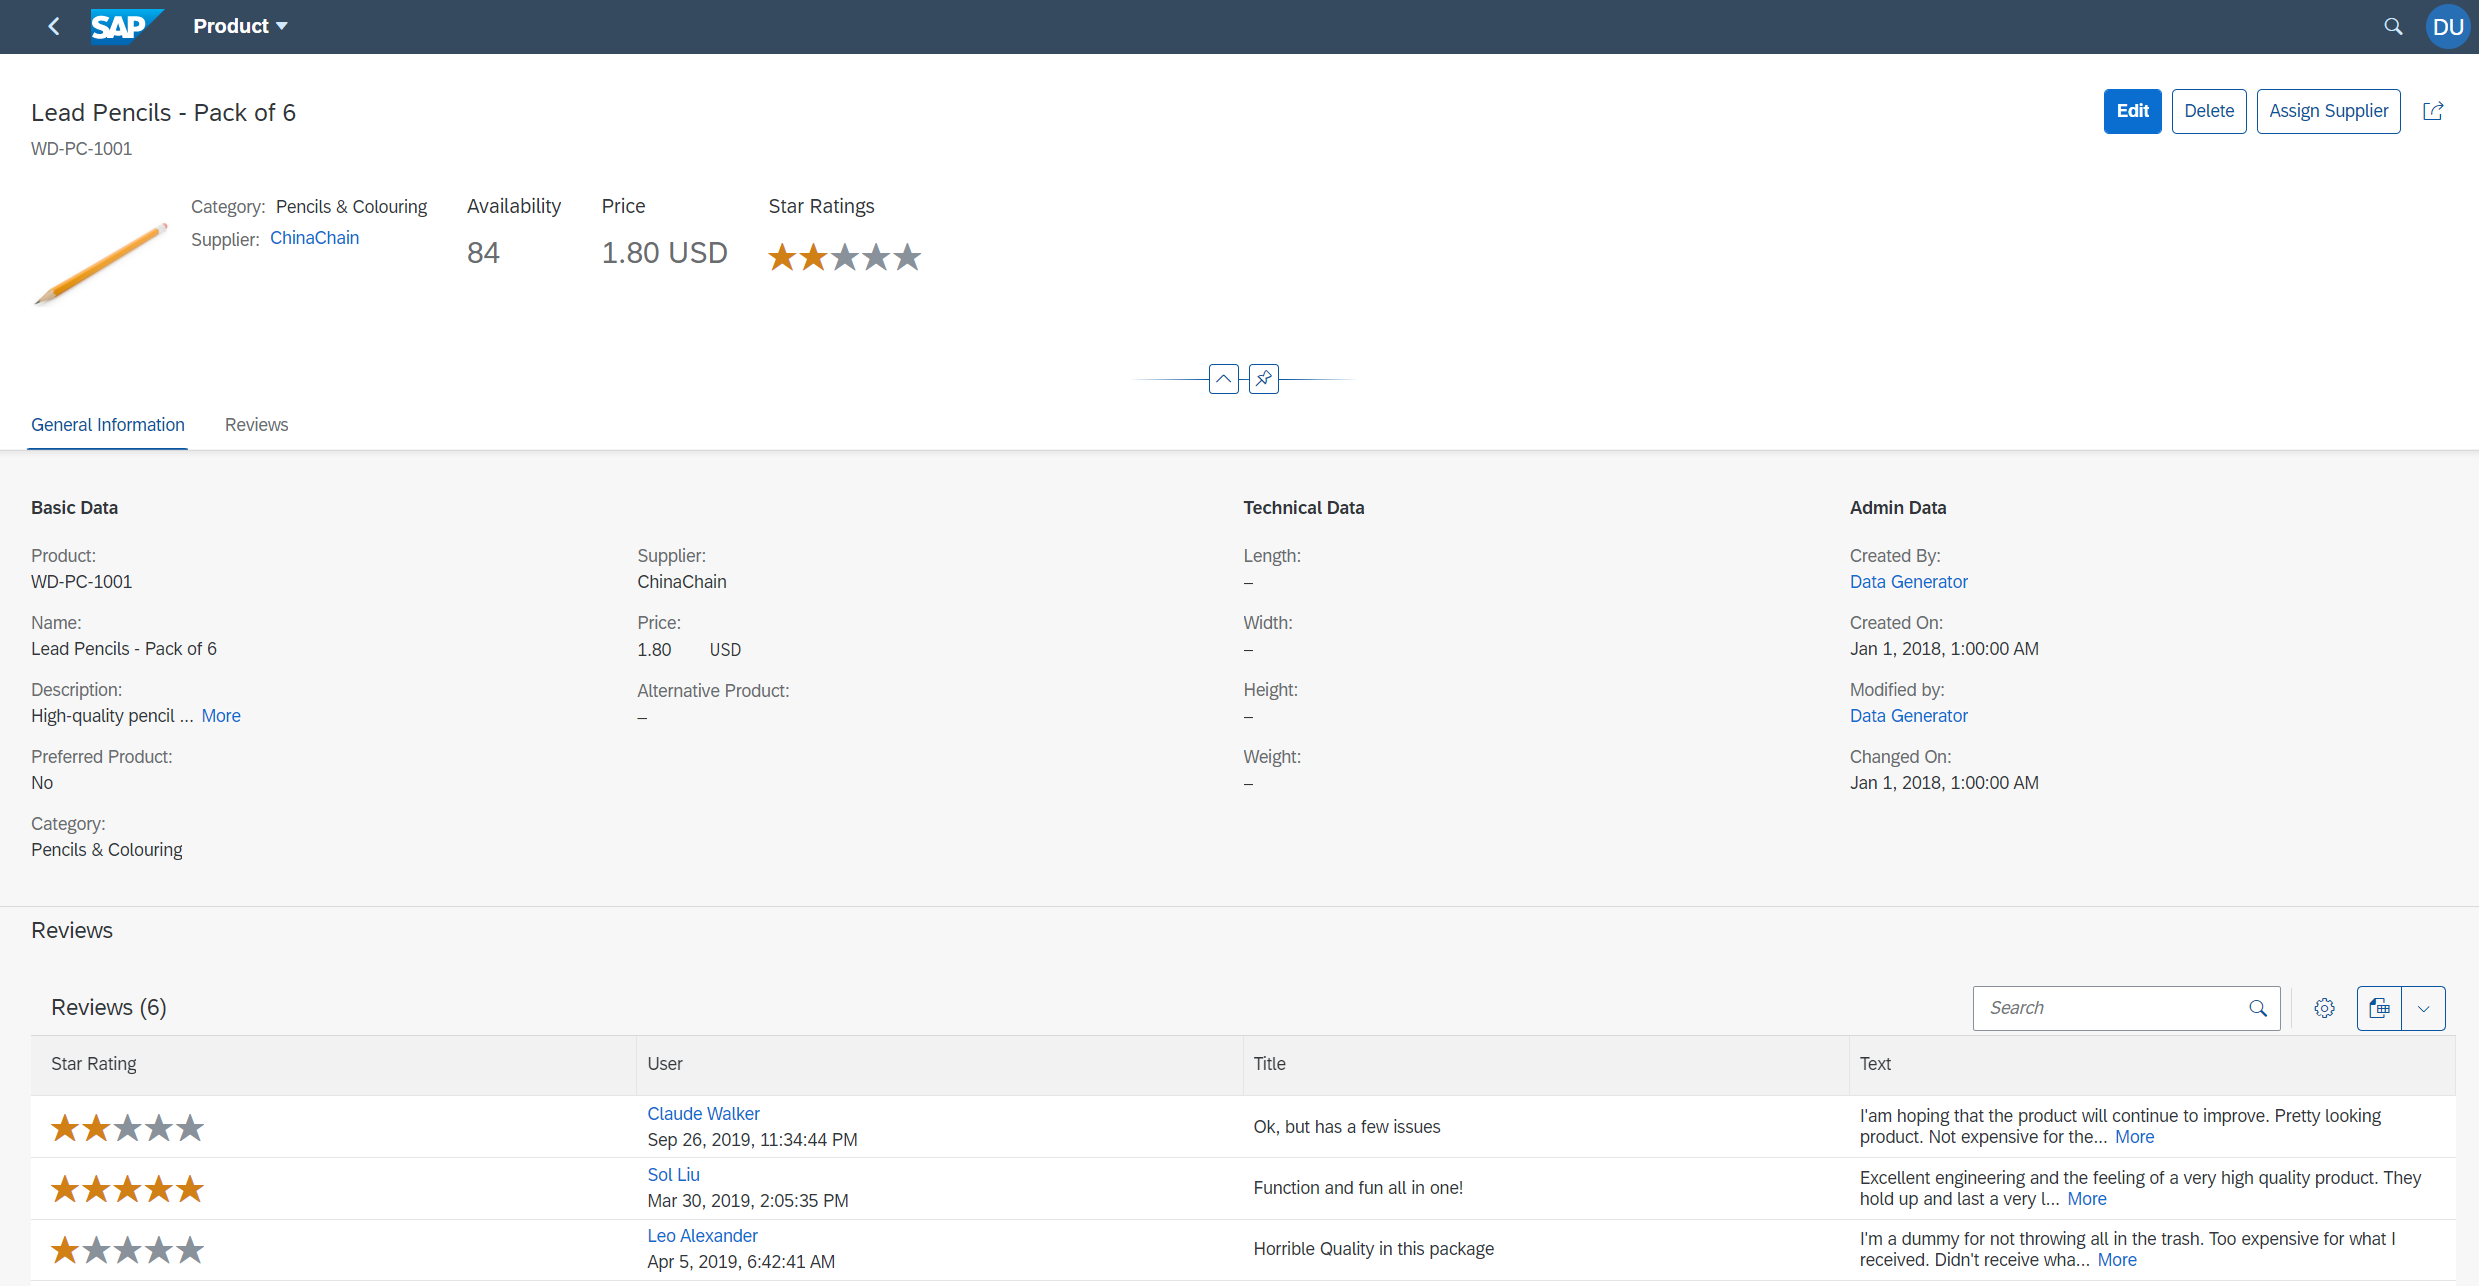
\includegraphics[height=6cm]{Bilder/Fiori_Elements_Object_Floorplan.png}
    \caption[Fiori Elements Object Page Floorplan]{Fiori Elements Object Page Floorplan}
    \label{fig:iso_norm}
\end{figure}

Das List Report Layout wird häufig mit der dem Object Page Floorplan in einer App kombiniert, wenn es darum geht, mit den einzelnen Objekten in der Liste zu arbeiten. Die Objekt-Ansicht wird durch einen Klick auf das gewünschte Objekt in der Listen-Ansicht aufgerufen. Hier können dann weitere Informationen zu \zB einem Produkt angezeigt und bei Bedarf auch bearbeitet werden. Des Weiteren gibt es noch Floorplans für eine Worklist, eine Liste mit Unterstützung für diverse Analyseverfahren, wie \zB Drill-Down und ein Dashboard.